
\section{Description of the model}
\label{sec:model}

In this section, the mathematical framework is described. The equations describing the evolution of the population categories are presented in Section~\ref{ssec:math}. The current implementation of the equations are validated against the results in literature in Section~\ref{ssec:literature}.

\subsection{Mathematical background}
\label{ssec:math}
The notation and the model used in this text is taken from reference \cite{MingLiu}. In this section, a brief overview, necessary to understand the document, is given. As mentioned in the introduction, the mathematical model is SEIQRS in a Small-Wolrd approximation. The population of $N$ individuals is separated into five classes: Susceptible, Exposed, Infected, Quarantined and Recovered. In the following, variables noted with capital letters (such as $S$, $E$\dots) indicate the absolute numbers of individuals belonging to the given category, whether quantities given in lowercase letters (such as $s$, $e$\dots) correspond to fractions of total populations (i.e. $s = S/N$). \\

The suscpetible $S$ category contain all people that may be potentially infected. They decrease in time, since people get exposed (with contact with an infected individual). However, healed people not developing immunity pass from the recovered category to the susceptible. The change in time of $s$, $\dot{s} = \frac{ds}{dt}$, is:
\begin{equation}
\dot{s} (t)= -\beta\braket{k}s(t)i(t)+\gamma{r(t)} 
\end{equation} 
The exposed $E$ category consist in susceptible individuals got in touch with an infected. An exposed person, after $\tau$ days, turn into infected. The equation for the variation in time of $e$, $\dot{e}$, is:
\begin{equation}
\dot{e} (t)= \beta\braket{k}s(t)i(t) - \beta\braket{k}s(t-\tau)i(t-\tau) 
\end{equation} 
Once an exposed person becomes infected, belonging to $I$, it may either die or being quarantined, resulting in the following equation for the variation in time of $i$, $\dot{i}$ :
\begin{equation}
\dot{i} (t)= \beta\braket{k}s(t-\tau)i(t-\tau) - d_1i(t) - \delta {i(t)}
\label{eqn:idot}
\end{equation} 
Quarantined people $Q$ may die or recover, therefore the variation of the quarantined category fraction $\dot{q}$ follows the equation:
\begin{equation}
\dot{q} = \delta{i(t)} - d_2{i(t)} - \mu{i(t)}
\end{equation}
Eventually, recovered people may actually turn back into susceptible  if they do not develop immunity. Therefore the equation for the variation of $r$ category, $\dot{r}$, is:
\begin{equation}
\dot{r} = \mu{q(t)}-\gamma{r(t)}
\end{equation}

The small-world assumption makes all individuals interact with each other. The number of interactions per day is measured by the $\braket{k}$ parameter. The initial conditions are $i(0) = i_0 \ll 1$, $e(0) = e_0 = \braket{k}i_0$ and $s(0) = s_0 = 1-i_0-e_0$. The coupled equations are solved with a second-order Runge-Kutta Method. No substantial discrepancy has been observed by the use of the Euler method.


\subsection{Validation against literature}
\label{ssec:literature}
The obtained results from the solution of equations above are cross-checked with the literature \cite{MingLiu,MingLiuOld}. The input parameters are set the same as in Section~4.1 of reference \cite{MingLiu}, where a numerical example of the model prediction is shown. The values of the parameters are reported in Table~\ref{tab:literature_parameters}.\\

\begin{table}
\centering
\begin{tabular}{@{}llllll@{}}
%\cmidrule[\heavyrulewidth]{1-2} \cmidrule[\heavyrulewidth]{4-5}
\toprule
%Parameter & Value & \phantom{aaa} & Parameter & Value \\
\multicolumn{5}{l}{Values of parameters in literature}\\
%\cmidrule{1-2} \cmidrule{4-5}
\midrule
$\beta$ & $2\times10^{-5}$ & \phantom{aaa} & $\braket{k}$ & $6$ \\
$\gamma$ & $2\times10^{-4}$ & \phantom{aaa} & $\delta$ & $0.3$ \\
$d_1$ & $5\times10^{-3}$ & \phantom{aaa} & $d_2$ & $1\times10^{-3}$ \\
$\tau$ & $5$ & \phantom{aaa} & & \\ [2mm]
$N$ & $10^4$ & \phantom{aaa} & $i_0$ & $1\times10^{-3}$\\
%\cmidrule[\heavyrulewidth]{1-2} \cmidrule[\heavyrulewidth]{4-5}
\bottomrule
\end{tabular}
\caption{Set of parameters used in Section~4.1 in reference \cite{MingLiu,MingLiuOld}.}
\label{tab:literature_parameters}
\end{table}

The evolution of the population categories obtained by solving the set of coupled equation in Section~\ref{ssec:math} is shown in Figure~\ref{fig:model_literature}. A clear difference of the evolution of the populations is evident with respect to figures in reference \cite{MingLiu}, where the outbreak actually occurs with a peak of about $20\%$ of population infected after $35$ days. The results with the implementation used in this document, the infected population dies down in about ten days. The motivation is that the initial infected population is not high enough with respect to the outbreak parameter ($\beta\braket{k}$) and the fraction of quarantined people. \\

The obtained behaviour of the outbreak is actually expected from the used equations, shown in Section~\ref{sec:model}. A necessary condition to let the outbreak spread is a positive increase of the infected population, so $\dot{i}(0)>0$. This provides an equation connecting the model parameters and the initial conditions:

\begin{equation}
i_0 > \frac{\left(\delta+d_1\right)-\beta\braket{k}}{\beta\braket{k}(1+\braket{k})}
\label{eqn:i0dotgtr0}
\end{equation}

Therefore, there is a threshold to the initial infected population to make the outbreak occur. From the Equation~\ref{eqn:i0dotgtr0}, a higher quarantine fraction and mortality ask for higher initial infected population. Also, since $\beta\braket{k}\ll\left(\delta+d_1\right)$, a smaller $\beta\braket{k}$ asks for higher initial infected population. Setting the model parameters to Table~\ref{tab:literature_parameters}, the minumum initial fraction of infected people $i_0>360$, meaningless, since it is expected to be lower than $1$. By imposing this condition, a relation between the different parameters is also found: 
\begin{equation}
\beta > \frac{\delta + d_1}{\braket{k}(\braket{k}+2)}
\label{eqn:i0low1}
\end{equation}
This condition is necessary to provide meaningful values of the population fractions. Using $\delta$, $d_1$ and $\braket{k}$ from Table~\ref{tab:literature_parameters}, the conditions in Equations~\ref{eqn:i0dotgtr0,eqn:i0low1} are $\beta>6\times10^{-3}$ and $i_0\approx1$, that is a limit case. An explaination of the discrepancy with respect to the literature is that probably the $\beta$ parameter is scaled up of orders of magnitudes according with the initial conditions or the total population. To find a reasonable set of parameters, the $\beta$ parameter is changed while all the other parameters to Table~\ref{tab:literature_parameters}. Since one wants $i_0\ll1$, then:

\begin{equation}
i_0<1 \Rightarrow \beta\gg \frac{\delta + d_1}{\braket{k}(\braket{k}+2)} \approx \frac{\delta}{\braket{k}(\braket{k}+2)} \approx \frac{0.3}{48} \approx 6\times10^{-3}
\label{eqn:numerical_i0low1}
\end{equation}

But also: 

\begin{equation}
\dot{i}(0)>1 \Rightarrow \beta > \frac{\delta + d_1}{\braket{k}\left[1+\left(1+\braket{k}\right)i_0\right]} \approx \frac{\delta}{\braket{k}} \approx \frac{0.3}{6} \approx 5\times10^{-2}
\label{eqn:numerical_i0dotgtr1}
\end{equation}

Assuming the difference is a matter of order of magnitude in the $\beta$ parameter, $\beta$ is set to $0.2$ ($N$ times the original value). The corresponding evolution is shown in Figure~\ref{fig:model_literature_modified}: a similar evolution as in reference  \cite{MingLiu} is finally obtained.

\begin{figure}[!ht]\centering
\subfloat[\label{fig:model_literature}
]{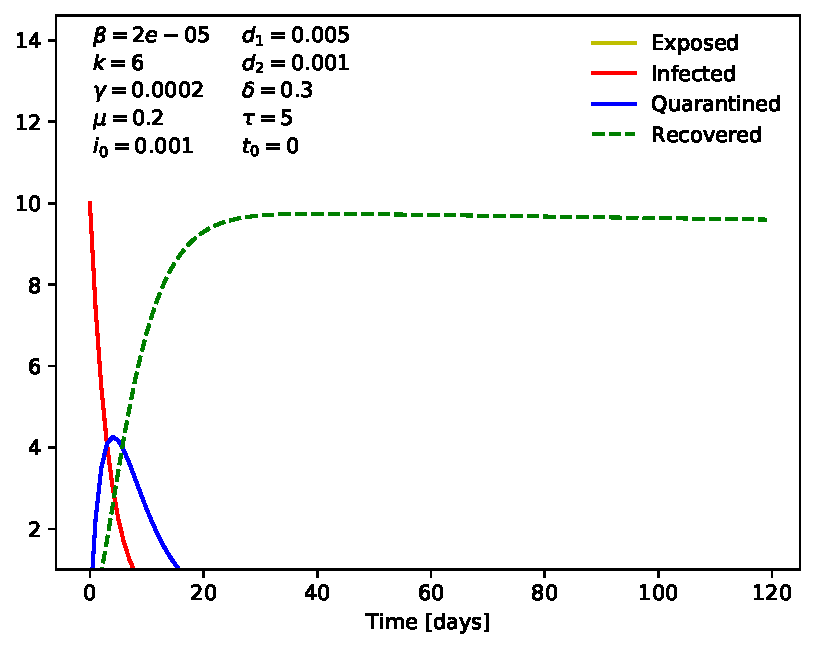
\includegraphics[width=0.4\textwidth]{imgs/ModelDescription/Summary_parameters_nominal.pdf}}
\subfloat[\label{fig:model_literature_modified}
]{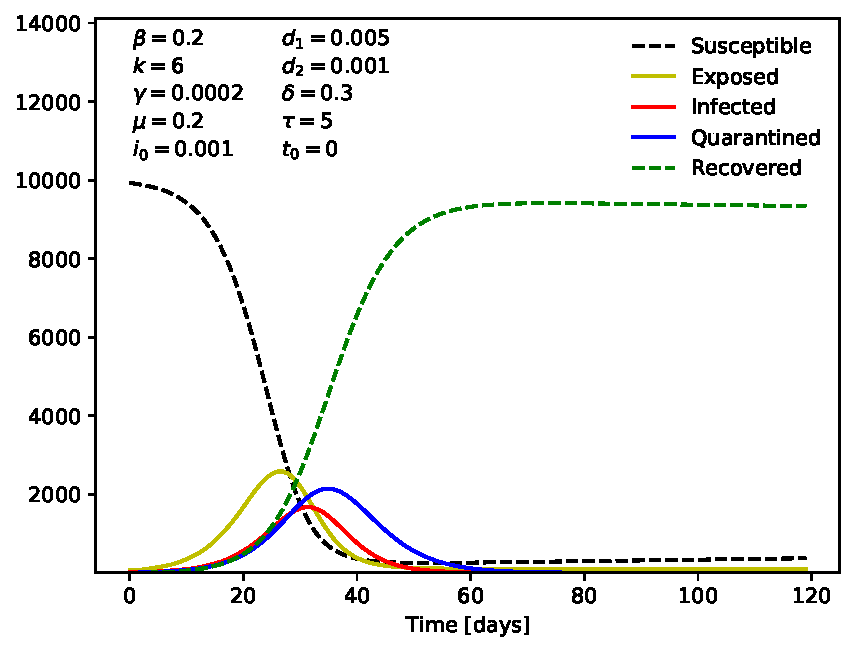
\includegraphics[width=0.42\textwidth]{imgs/ModelDescription/Summary_parameters_alternative.pdf}}
\caption{Numerical prediction of the model with different settings of the parameters. Parameters in Table~\ref{tab:literature_parameters} are used in (a), as well as in (b) but for $\beta$ parameter set to $0.2$.}.
\end{figure}



